\documentclass{alex_hü}

\name{Alexander Helbok}
\course{PS Physik}
\hwnumber{4}


\begin{document}
\renewcommand{\labelenumi}{(\alph{enumi})}


\begin{mybox}{1. Der Dipol}
	\centering \(k = \tfrac{1}{4\pi \epsilon_0};\quad x_1 = -\tfrac{d}{2};\quad x_2 = \tfrac{d}{2} \)
	\tcblower
	\begin{enumerate}
		\item \(  \)
			\( V_{ges} = V_+ + V_- = kq\left(\tfrac{1}{r_+} - \tfrac{1}{r_-} \right)\\[1em] \)
			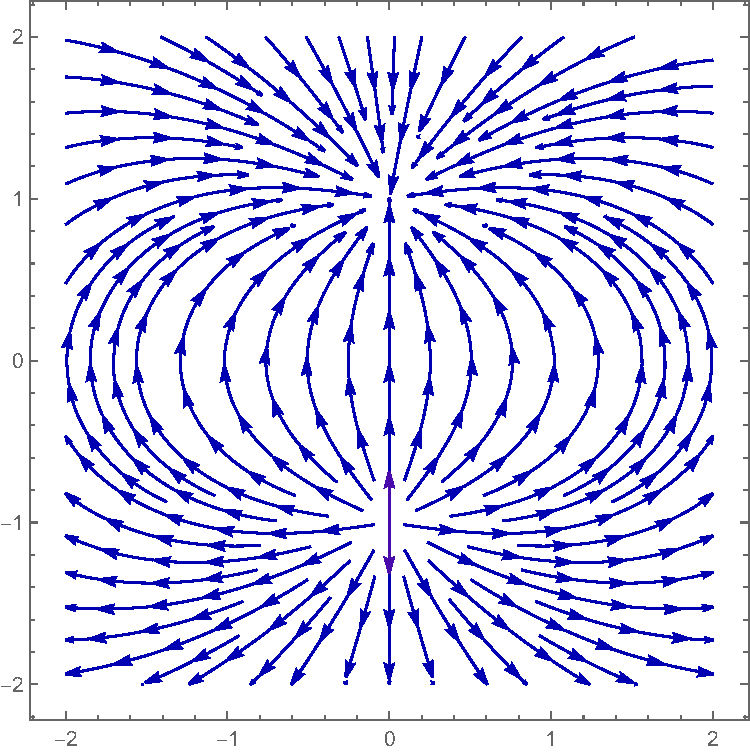
\includegraphics[scale=0.7]{dipole.pdf}
	\tcbline
		\item \( d \ll r;\quad \vec{p} := q\vec{d};\quad d\cos(\theta) = \vec{d} \)
		\begin{flalign*}
			V &= kq\left(\tfrac{1}{r_+} - \tfrac{1}{r_-} \right) = kq\left(\tfrac{r_- - r_+}{r_+r_-} \right) \approx kq\tfrac{d\cos(\theta)}{r^2} &&\\
			&= k \frac{p\cos(\theta)}{r^2} = \dl{k \frac{\vec{p} \cdot \vec{r}}{r^3}} &&
		\end{flalign*}
		\hfill
		\begin{minipage}[t]{0.3\textwidth}
			\vspace{-2.3cm}
			\boxed{
				\begin{aligned}
					r_- - r_+ &\approx d\cos(\theta) \\
					r_+r_- \pm l &\approx r^2
				\end{aligned}
			}
		\end{minipage}\\
	\tcbline
		\item \( \abs*{\vec{M}} = \abs*{\vec{p} \times \vec{E}} = pE\sin(\theta);\quad E_{pot} = \int\limits_{\theta}^{\pi/2}\ \abs*{\vec{M}}\ \mathrm{d}\tilde{\theta} \)
		\begin{flalign*}
			E_{pot} &= \uint[\theta,\pi/2]{\abs*{\vec{M}}}{\tilde{\theta}} = pE \uint[\theta,\pi/2]{\sin(\tilde{\theta})}{\tilde{\theta}} = pE\cos(\theta) &&\\
			&= \dl{\vec{p} \cdot \vec{E}} &&
		\end{flalign*}
	\end{enumerate}
\end{mybox}

\begin{mybox}{2. Kondensator mit Dielektrikum}
	\centering \(k = \tfrac{1}{4\pi \epsilon_0};\quad C = \tfrac{\epsilon A}{d};\quad \epsilon_{rel} = \tfrac{\epsilon}{\epsilon_0} \)
	\tcblower
	\begin{enumerate}
		\item \(  \)
		\begin{flalign*}
			C_1 &= \tfrac{\epsilon_0 a(a-h)}{d} &&\\
			C_2 &= \tfrac{\epsilon_r ah}{d} &&\\
			C_{ges} &= C_1 + C_2 = \dl{\tfrac{\epsilon_0 a}{d}\left(\epsilon_{rel}h + a - h \right)} &&
		\end{flalign*}
	\tcbline
		\item \(  \)
		\begin{flalign*}
			E &= \tfrac{CU^2}{2} = \dl{\tfrac{U^2\epsilon_0 a(\epsilon_{rel}h + a - h)}{2d}} &&
		\end{flalign*}
	\tcbline
		\item \(  \)
		\begin{flalign*}
			E' &= \tfrac{C'U^2}{2} = \tfrac{U^2\epsilon_0 a(\epsilon_{rel}(h + \Delta h) + a - (h + \Delta h))}{2d} &&\\
			\Delta E &= \dl{\tfrac{U^2\epsilon_0 a}{2d}(\epsilon_{rel}\Delta h - \Delta h)} &&\\[2em]
			E_{pot} &= \tfrac{mgh}{2} = \tfrac{\rho adgh^2}{2} &&\\
			E_{pot}' &= \tfrac{\rho adg(h + \Delta h)^2}{2} &&\\
			\Delta E_{pot} &= \dl{\tfrac{\rho g a d}{2}(\Delta h^2 + 2h\Delta h)} &&
		\end{flalign*}
	\tcbline
		\item \(  \)
		\begin{flalign*}
			\Delta q &= 2\tfrac{\Delta E}{U} = \dl{\tfrac{U\epsilon_0 a}{d}(\epsilon_{rel}\Delta h - \Delta h)} &&
		\end{flalign*}
	\tcbline
		\item \(  \)
	\tcbline
		\item \( a = 0.1 \unit{m};\quad d = 5.0 * 10^{-3}\unit{m};\quad h = 0.05 \unit{m};\quad U = 7 \unit{kV}\\ \epsilon_r = 80;\quad \rho = 1.0 * 10^{3}\unit{kg/m^3}\)
		\begin{flalign*}
			C_{ges} &= C_1 + C_2 = \tfrac{\epsilon_0 a}{d}\left(\epsilon_{rel}h + a - h \right) = \dl{7.17 * 10^{-10} \unit{F}} &&\\[1.5em]
			E_{pot} &= \tfrac{mgh}{2} = \dl{6.1 * 10^{-3} \unit{J}} &&
		\end{flalign*}
	\end{enumerate}
\end{mybox}

\begin{mybox}{3. Kapazität eines Koaxialkabels}
	\centering \(k = \tfrac{1}{4\pi \epsilon_0};\quad C = \tfrac{\epsilon A}{d};\quad \epsilon_{rel} = \tfrac{\epsilon}{\epsilon_0} \)
	\tcblower
	\begin{enumerate}
		\item \(  \)
		\underline{For  \(r \leq d \leq R\):}
		\begin{flalign*}
			\frac{q_{in}}{\epsilon_0} &= \oint \vec{E}(\vec{d})\ \mathrm{d}\vec{A} = E(d) \oint \mathrm{d}A = E(d)2\pi dl &&\\
			E(d) &= kq \tfrac{2}{dl} &&\\
		\end{flalign*}
		\underline{For \(R < d\):}
		\begin{flalign*}
			q_{in} &= 0 &&\\
			E(d) &= 0 &&
		\end{flalign*}
		\boxed{
			\begin{aligned}
				E(d) = \begin{cases}
					kQ \tfrac{2}{lr}& \quad $for $\ r \leq d \leq R, \\
					0& \quad $for $\ R < d. 
				\end{cases} 
			\end{aligned}
		}
	\tcbline
		\item \(  \)
%		\underline{For \(R < d\):}
%		\begin{flalign*}
%			E(d) &= 0 &&\\
%			V(d) &= \int\limits_{d}^{\infty}\ \vec{E}(r)\ \mathrm{d}\vec{r} = 0 &&
%		\end{flalign*}
		\underline{For  \(r \leq d \leq R\):}
		\begin{flalign*}
			E(d) &= kq \tfrac{2}{dl} &&\\
			V(d) &= \uint[d,\infty]{\vec{E}(r)}{r} = \uint[d,R]{kq \tfrac{2}{rl}}{r} + \tikzmark{1} \uint[R,\infty]{0}{r} \tikzmark{2} &&\\[2em]
			V(d) &= \tfrac{2kq}{l}\ln(\tfrac{R}{d})  &&\\
		\end{flalign*}
	\AddUnderBrace[2.2em]{1}{2}{$= 0$}
		\boxed{
			\begin{aligned}
				V(d) = \begin{cases}
					\tfrac{2kq}{l}\ln(\tfrac{R}{d})& \quad $for $\ r \leq d \leq R, \\
					0& \quad $for $\ R < d. 
				\end{cases} 
			\end{aligned}
		}
	\tcbline
		\item \( r = 7.0 * 10^{-4} \unit{m};\quad R = 2.5 * 10^{-3} \unit{m};\quad C = 500 \unit{pF} \)
		\begin{flalign*}
			C &= \frac{q}{V(r)} = \tfrac{l}{2k\ln(\tfrac{R}{r})} &&\\
			l &= \tfrac{C}{2k\ln(\tfrac{R}{r})} &&\\
			&= \dl{11.44 \unit{m}} &&
		\end{flalign*}
	\tcbline
		\item \( I = 0.1 \unit{A};\quad U = 10 \unit{V} \)
		\begin{flalign*}
			t &= \tfrac{CU}{I} = \dl{50 \unit{ns}} &&
		\end{flalign*}
	\end{enumerate}
\end{mybox}

\end{document}